\lhead{\emph{Arquitectura}}
\chapter{Arquitectura}

Sumada a las herramientas creadas en el sistema, es necesario llevar a cabo una serie de operaciones que posibiliten el acceso a servicios más básicos tales como la autenticación de los usuarios del sistema, %TODO etc

Con el objetivo de mejorar la situación actual en la infraestructura a analizar, se tratan los siguientes problemas.

\section{Instalación del sistema}

El sistema a crear requiere de la instalación de diferentes componentes, en particular el sistema operativo, antes de poder ser utilizado. Dicha instalación, si es realizada en cada nodo secuencialmente, implica una gran carga de trabajo y aumenta la propensión a errores durante dicho proceso (en particular si en el mismo existe una gran carga de trabajo que debe ser supervisado por un administrador humano). Una solución a este problema es la autoinstalación del sistema operativo partiendo de una imagen definida y probada por el administrador, que se cargará e instalará en cada nodo sin supervisión.

Una de las herramientas ya existentes para solucionar este problema es el \textbf{PXE} (\textit{Preboox eXecution Environment})\cite{pxeintel}, un estándar \textit{de facto}\cite{avramov:architecture} para la carga de un sistema operativo desde un servidor. El estándar se apoya en protocolos presentes en la práctica totalidad de sistemas, tales como \textbf{DHCP}, \textbf{TFTP} y \textbf{TCP/IP}. El descubrimiento de servicios se realiza mediante una extensión en el mensaje \textbf{DHCPDISCOVER} que envía el servicio \textbf{DHCP} en su secuencia de arranque\cite{rfc4578}. El servidor \textbf{DHCP}, si implementa esta extensión del protocolo, enviará la información sobre la localización de cada uno de los servidores de arranque al cliente, que procederá a la descarga utilizando el protocolo \textbf{TFTP} y posterior instalación\cite{pxeoverview}.

Sin embargo, el uso de este protocolo requiere un controlador de interfaz de red (\textbf{NIC}) en el cliente que soporte el protocolo \textbf{PXE}. Generalmente dicho controlador se incluye como extensión de la \textbf{BIOS} o en equipos más modernos como código \textbf{UEFI}. La \textbf{Raspberry Pi} carece de este tipo de \textit{software}, pues delega todo el arranque del sistema a los datos presentes en la tarjeta SD, y por tanto no es posible realizar ningún tipo de arranque en red sin la previa instalación de un conjunto de aplicaciones que realicen la descarga del sistema operativo. Es por ello que el uso de \textbf{PXE} como herramienta de arranque debe ser desestimado.

\subsection{marco-netinst}

Debido a la falta de soporte para \textbf{PXE} u otra alternativa similar, es necesario crear una herramienta que se encargue de la detección de un servidor que aloje la imagen del sistema operativo, la descarga del mismo y su instalación. Con este objetivo se crea la herramienta \textbf{marco-netinst}.

\textbf{marco-netinst} es una ramificación del proyecto \textbf{rasbpian-ua-netinst}\cite{raspbian-ua-netinst}. Esta utilidad permite instalar un conjunto mínimo de utilidades que posibilitan la descarga de un sistema operativo desde los repositorios de \textbf{Debian} y su instalación. La ramificación incluye las siguientes modificaciones:

\begin{itemize}
	\item Instalación de \textbf{ArchLinux ARM} en lugar de \textbf{Raspbian}.
	\item Instalación del sistema operativo completo a partir de un archivo \textbf{.tar.gz} en lugar de la descarga de paquetes\footnote{\textbf{raspbian-ua-netinst} utiliza el paquete cdebootstrap-static para la descarga e instalación de todos los archivos. Existe una herramienta para ArchLinux similar, denominada \textbf{Archbootstrap}\\
	\href{https://wiki.archlinux.org/index.php/Archbootstrap}{https://wiki.archlinux.org/index.php/Archbootstrap}\\
	\href{https://packages.debian.org/sid/cdebootstrap-static}{https://packages.debian.org/sid/cdebootstrap-static}}.
	\item Nuevo \textit{script} de carga del \textit{software} en la tarjeta SD (en el paquete original se delega a utilidades de terceros).
	%TODO\item Posibilidad de aplicar diferentes esquemas de particionado
	\item Detección del servidor sin configuración previa utilizando \textbf{MarcoPolo}.
	%TODO\item Interfaz administrativa de los sistemas operativos ofrecidos
\end{itemize}

La especificación en detalle del funcionamiento de la herramienta se detalla en el anexo%TODOf

\section{Autenticación de los usuarios}

Los usuarios del sistema deben ser capaces de acceder al sistema mediante un sistema de credenciales que posibilite el uso de cualquier nodo del sistema con el mismo conjunto de claves. Dicho enfoque es el propio de la infraestructura actual del sistema, que en concreto sigue un enfoque centralizado.

Un primer intento de posibilitar la ``universalización'' del acceso ha sido la creación de los mismos usuarios en cada uno de los nodos, utilizando el mismo par usuario-contraseña en cada uno de ellos. Sin embargo, este enfoque impide una escalabilidad sencilla y requiere un mantenimiento continuo (suponiendo que se añaden usuarios periódicamente). Por ello únicamente las pruebas iniciales de las plataformas que requieren acceso a la funcionalidad de autenticación han sido realizadas siguiendo este enfoque, pero siempre desacoplando al máximo el sistema de acceso del resto de la lógica del programa, con el objetivo de facilitar su reemplazo.

Habiendo descartado dicha estrategia, queda como alternativa más adecuada a las necesidades del sistema el uso de la infraestructura presente en el centro académico.

La infraestructura del centro comprende varios servicios que interactúan entre sí, siendo el pilar clave el servidor LDAP (\textit{Lightweight Directory Access Protocol})\citationneeded. Dicho servidor almacena la información de todos los usuarios de la infraestructura y da acceso a cualquier equipo de varias de las aulas de la Facultad.
\begin{figure}[H]
	\centering
	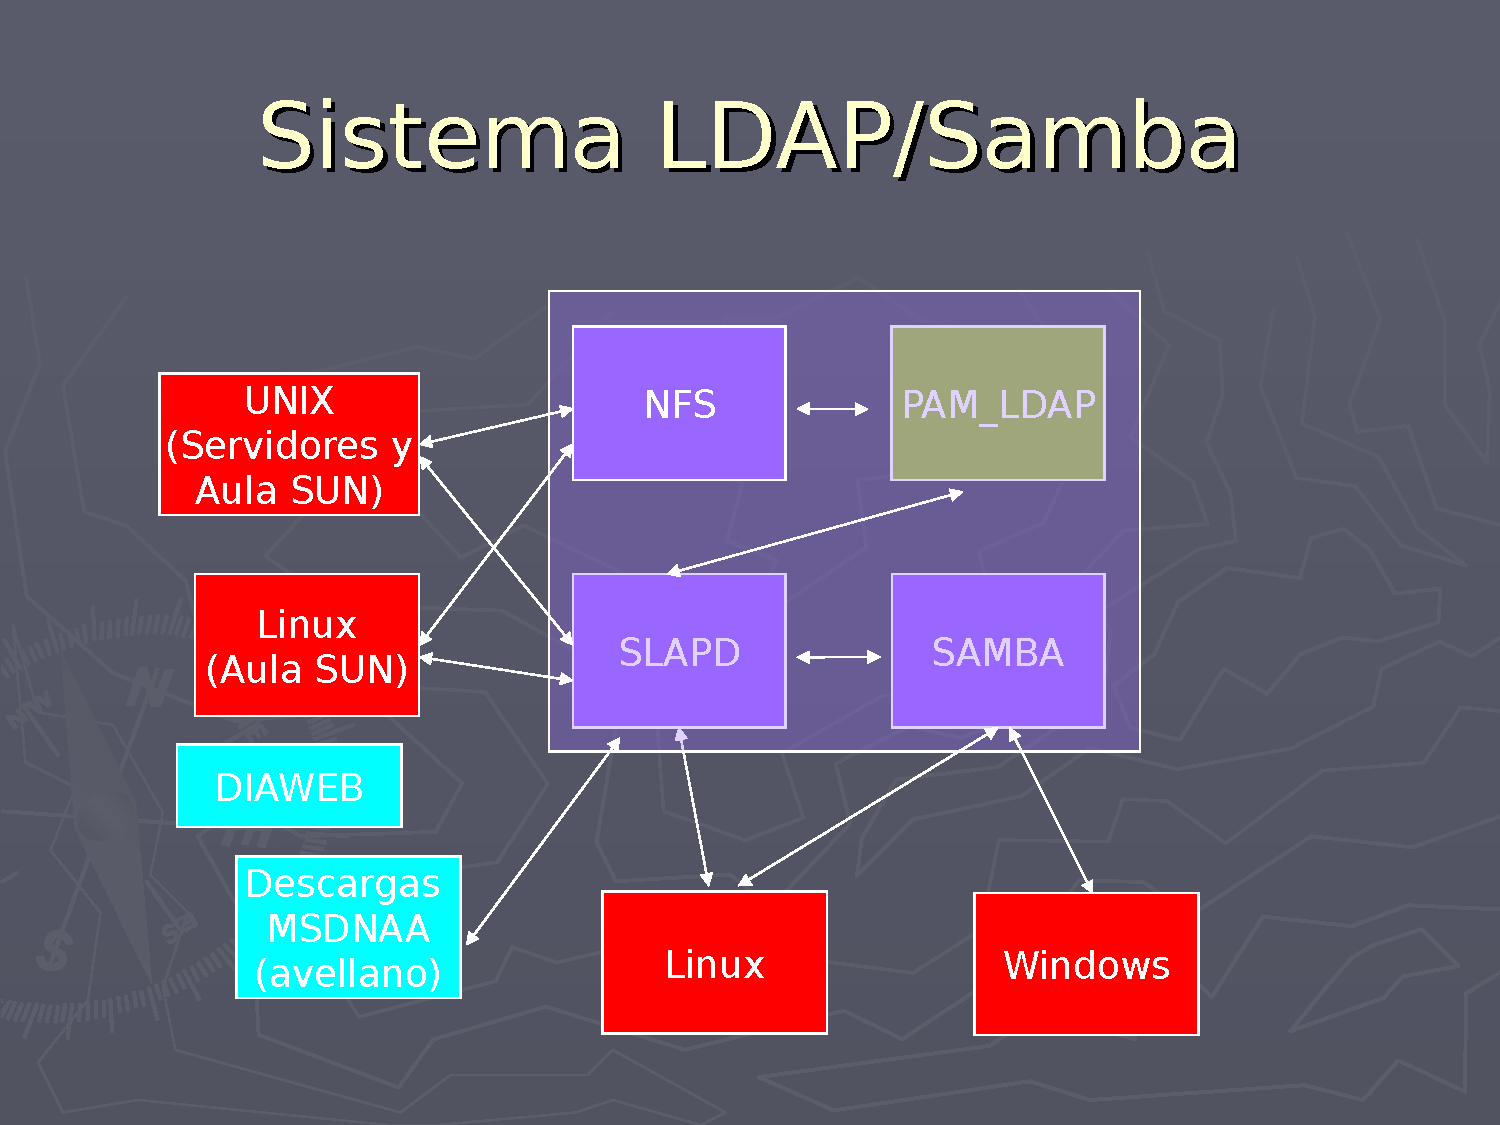
\includegraphics[width=0.7\textwidth]{Chapter4/Figures/LDAP.pdf}
	\caption{Esquema de los diferentes componentes del sistema de autenticación y gestión de archivos, así como de una serie de componentes adicionales. Obsérvese la interacción entre los componentes situados en el rectángulo interior}
	\label{fig:arquitectura_ldap}
\end{figure}

\subsection{Características en detalle}

Debido a la heterogeneidad de los diferentes equipos presentes en la infraestructura, el sistema debe posibilitar el acceso a todos los equipos utilizando el mismo conjunto de credenciales. Esto implica que el sistema debe ser compatible con al menos los sistemas operativos GNU/Linux, Microsoft Windows y Solaris. Por ello se interconecta el servidor LDAP con Samba, así como el PAM (\textit{Pluggable Authentication Module}) tanto en el cliente como el servidor.

Sin embargo el sistema permite también que los usuarios puedan almacenar información en un espacio centralizado al que es posible acceder desde cualquier equipo, facilitando la copia de ficheros entre nodos, uniformidad de los diferentes equipos. Esto se consigue utilizando un servidor NFS (\textit{Network File Storage}).

\subsection{Utilización en el sistema}

En el sistema se aprovechará principalmente la funcionalidad de autenticación provista por el servidor LDAP, debido a que uno de los objetivos principales del sistema es evitar ``cuellos de botella'' debido al uso de un servidor de almacenamiento central. Herramientas como el \textbf{deployer} facilitarán la replicación de servicios en su lugar. En cualquier caso, se plantea permitir el acceso al NFS desde el sistema como complemento, pero no como espacio principal de almacenamiento.

El sistema aprovecha el módulo PAM para realizar el proceso de autenticación.

\section{Compilación}

Si bien el sistema Raspberry Pi es capaz de compilar el \textit{software} que después utilizará, en ocasiones es beneficioso delegar dicha tarea a otro componente que realice el proceso por el nodo en cuestión y posteriormente añadir los archivos ejecutables al sistema. Este enfoque reduce el tiempo de trabajo de forma significativa, como observaremos posteriormente.%proporcione los resultados al solicitante.

\subsection{Creación de un compilador cruzado}

Un compilador cruzado (\textit{cross-compiler})es una herramienta capaz de generar código para una architectura utilizando un equipo con otra arquitectura diferente.%TODO: http://en.wikipedia.org/wiki/Cross_compiler
El uso de compiladores cruzados 